% Options for packages loaded elsewhere
\PassOptionsToPackage{unicode}{hyperref}
\PassOptionsToPackage{hyphens}{url}
%
\documentclass[
]{article}
\usepackage{amsmath,amssymb}
\usepackage{lmodern}
\usepackage{iftex}
\ifPDFTeX
  \usepackage[T1]{fontenc}
  \usepackage[utf8]{inputenc}
  \usepackage{textcomp} % provide euro and other symbols
\else % if luatex or xetex
  \usepackage{unicode-math}
  \defaultfontfeatures{Scale=MatchLowercase}
  \defaultfontfeatures[\rmfamily]{Ligatures=TeX,Scale=1}
\fi
% Use upquote if available, for straight quotes in verbatim environments
\IfFileExists{upquote.sty}{\usepackage{upquote}}{}
\IfFileExists{microtype.sty}{% use microtype if available
  \usepackage[]{microtype}
  \UseMicrotypeSet[protrusion]{basicmath} % disable protrusion for tt fonts
}{}
\makeatletter
\@ifundefined{KOMAClassName}{% if non-KOMA class
  \IfFileExists{parskip.sty}{%
    \usepackage{parskip}
  }{% else
    \setlength{\parindent}{0pt}
    \setlength{\parskip}{6pt plus 2pt minus 1pt}}
}{% if KOMA class
  \KOMAoptions{parskip=half}}
\makeatother
\usepackage{xcolor}
\IfFileExists{xurl.sty}{\usepackage{xurl}}{} % add URL line breaks if available
\IfFileExists{bookmark.sty}{\usepackage{bookmark}}{\usepackage{hyperref}}
\hypersetup{
  pdfauthor={Eitan \& Yuval Bakirov},
  hidelinks,
  pdfcreator={LaTeX via pandoc}}
\urlstyle{same} % disable monospaced font for URLs
\usepackage[margin=1in]{geometry}
\usepackage{color}
\usepackage{fancyvrb}
\newcommand{\VerbBar}{|}
\newcommand{\VERB}{\Verb[commandchars=\\\{\}]}
\DefineVerbatimEnvironment{Highlighting}{Verbatim}{commandchars=\\\{\}}
% Add ',fontsize=\small' for more characters per line
\usepackage{framed}
\definecolor{shadecolor}{RGB}{248,248,248}
\newenvironment{Shaded}{\begin{snugshade}}{\end{snugshade}}
\newcommand{\AlertTok}[1]{\textcolor[rgb]{0.94,0.16,0.16}{#1}}
\newcommand{\AnnotationTok}[1]{\textcolor[rgb]{0.56,0.35,0.01}{\textbf{\textit{#1}}}}
\newcommand{\AttributeTok}[1]{\textcolor[rgb]{0.77,0.63,0.00}{#1}}
\newcommand{\BaseNTok}[1]{\textcolor[rgb]{0.00,0.00,0.81}{#1}}
\newcommand{\BuiltInTok}[1]{#1}
\newcommand{\CharTok}[1]{\textcolor[rgb]{0.31,0.60,0.02}{#1}}
\newcommand{\CommentTok}[1]{\textcolor[rgb]{0.56,0.35,0.01}{\textit{#1}}}
\newcommand{\CommentVarTok}[1]{\textcolor[rgb]{0.56,0.35,0.01}{\textbf{\textit{#1}}}}
\newcommand{\ConstantTok}[1]{\textcolor[rgb]{0.00,0.00,0.00}{#1}}
\newcommand{\ControlFlowTok}[1]{\textcolor[rgb]{0.13,0.29,0.53}{\textbf{#1}}}
\newcommand{\DataTypeTok}[1]{\textcolor[rgb]{0.13,0.29,0.53}{#1}}
\newcommand{\DecValTok}[1]{\textcolor[rgb]{0.00,0.00,0.81}{#1}}
\newcommand{\DocumentationTok}[1]{\textcolor[rgb]{0.56,0.35,0.01}{\textbf{\textit{#1}}}}
\newcommand{\ErrorTok}[1]{\textcolor[rgb]{0.64,0.00,0.00}{\textbf{#1}}}
\newcommand{\ExtensionTok}[1]{#1}
\newcommand{\FloatTok}[1]{\textcolor[rgb]{0.00,0.00,0.81}{#1}}
\newcommand{\FunctionTok}[1]{\textcolor[rgb]{0.00,0.00,0.00}{#1}}
\newcommand{\ImportTok}[1]{#1}
\newcommand{\InformationTok}[1]{\textcolor[rgb]{0.56,0.35,0.01}{\textbf{\textit{#1}}}}
\newcommand{\KeywordTok}[1]{\textcolor[rgb]{0.13,0.29,0.53}{\textbf{#1}}}
\newcommand{\NormalTok}[1]{#1}
\newcommand{\OperatorTok}[1]{\textcolor[rgb]{0.81,0.36,0.00}{\textbf{#1}}}
\newcommand{\OtherTok}[1]{\textcolor[rgb]{0.56,0.35,0.01}{#1}}
\newcommand{\PreprocessorTok}[1]{\textcolor[rgb]{0.56,0.35,0.01}{\textit{#1}}}
\newcommand{\RegionMarkerTok}[1]{#1}
\newcommand{\SpecialCharTok}[1]{\textcolor[rgb]{0.00,0.00,0.00}{#1}}
\newcommand{\SpecialStringTok}[1]{\textcolor[rgb]{0.31,0.60,0.02}{#1}}
\newcommand{\StringTok}[1]{\textcolor[rgb]{0.31,0.60,0.02}{#1}}
\newcommand{\VariableTok}[1]{\textcolor[rgb]{0.00,0.00,0.00}{#1}}
\newcommand{\VerbatimStringTok}[1]{\textcolor[rgb]{0.31,0.60,0.02}{#1}}
\newcommand{\WarningTok}[1]{\textcolor[rgb]{0.56,0.35,0.01}{\textbf{\textit{#1}}}}
\usepackage{longtable,booktabs,array}
\usepackage{calc} % for calculating minipage widths
% Correct order of tables after \paragraph or \subparagraph
\usepackage{etoolbox}
\makeatletter
\patchcmd\longtable{\par}{\if@noskipsec\mbox{}\fi\par}{}{}
\makeatother
% Allow footnotes in longtable head/foot
\IfFileExists{footnotehyper.sty}{\usepackage{footnotehyper}}{\usepackage{footnote}}
\makesavenoteenv{longtable}
\usepackage{graphicx}
\makeatletter
\def\maxwidth{\ifdim\Gin@nat@width>\linewidth\linewidth\else\Gin@nat@width\fi}
\def\maxheight{\ifdim\Gin@nat@height>\textheight\textheight\else\Gin@nat@height\fi}
\makeatother
% Scale images if necessary, so that they will not overflow the page
% margins by default, and it is still possible to overwrite the defaults
% using explicit options in \includegraphics[width, height, ...]{}
\setkeys{Gin}{width=\maxwidth,height=\maxheight,keepaspectratio}
% Set default figure placement to htbp
\makeatletter
\def\fps@figure{htbp}
\makeatother
\setlength{\emergencystretch}{3em} % prevent overfull lines
\providecommand{\tightlist}{%
  \setlength{\itemsep}{0pt}\setlength{\parskip}{0pt}}
\setcounter{secnumdepth}{-\maxdimen} % remove section numbering
\ifLuaTeX
  \usepackage{selnolig}  % disable illegal ligatures
\fi

\author{Eitan \& Yuval Bakirov}
\date{2022-06-09}

\begin{document}


\includegraphics{C:/Users/eitan/OneDrive/Desktop/TAU/Semester B/Statistics and Data Analysis/Happiness/World-Happiness-Report.png}

\begin{center}\rule{0.5\linewidth}{0.5pt}\end{center}

Eitan and Yuval Bakirov

June 2022

\begin{center}\rule{0.5\linewidth}{0.5pt}\end{center}

\hfill\break

\hypertarget{introduction}{%
\subsection{Introduction}\label{introduction}}

The World Happiness Report is a landmark survey of the state of global
happiness. The first report was published in 2012, the second in 2013,
the third in 2015, and the fourth in the 2016 Update. The World
Happiness 2017, which ranks 155 countries by their happiness levels, was
released at the United Nations at an event celebrating International Day
of Happiness on March 20th. The report continues to gain global
recognition as governments, organizations and civil society increasingly
use happiness indicators to inform their policy-making decisions.
Leading experts across fields -- economics, psychology, survey analysis,
national statistics, health, public policy and more -- describe how
measurements of well-being can be used effectively to assess the
progress of nations. The reports review the state of happiness in the
world today and show how the new science of happiness explains personal
and national variations in happiness.

\hfill\break

\hypertarget{goals}{%
\subsubsection{Goals}\label{goals}}

\begin{longtable}[]{@{}ll@{}}
\toprule
Table Header & Second Header \\
\midrule
\endhead
Table Cell & Cell 2 \\
Cell 3 & Cell 4 \\
\bottomrule
\end{longtable}

Our goal is to see the correlation between the happiness of countries to
other statistical data, such as, GDP per capita of each country, its'
healthy life expectancy, generosity etc.

\hfill\break
In our project we will focus on:\\

\begin{itemize}
\tightlist
\item
  Tidy our data set
\item
  Visualizations
\item
  Statistical Models and methods learned during the course\\
  \strut \\
\end{itemize}

The methods which we will use in this research are:

\begin{enumerate}
\def\labelenumi{\arabic{enumi}.}
\item
  Hypothesis test - difference in means - we want to test the assumption
  that the median happiness score went up over the years.\\
  For this reason we will perform a T-Test.
\item
  Model of multiple regression - we want to examine the effect of
  explanatory variables on the level of happiness (the explained
  variable). We will perform tests to draw conclusions using Summary
  Statistics Table.
\end{enumerate}

\hfill\break

\hypertarget{part-one---data-import-and-tidying}{%
\subsubsection{Part One - Data Import And
Tidying}\label{part-one---data-import-and-tidying}}

\hfill\break

\hypertarget{data-import}{%
\paragraph{Data import}\label{data-import}}

\begin{Shaded}
\begin{Highlighting}[]
\FunctionTok{library}\NormalTok{(tidyverse)}
\FunctionTok{library}\NormalTok{(gridExtra) }\CommentTok{\#for grid.arrange}
\FunctionTok{library}\NormalTok{(dplyr)}
\FunctionTok{library}\NormalTok{(corrplot)}
\FunctionTok{library}\NormalTok{(ggcorrplot) }\CommentTok{\#for correlation plot}
\FunctionTok{library}\NormalTok{(car)}

\CommentTok{\# install.packages("remotes")}
\CommentTok{\# remotes::install\_github("OHDSI/CohortMethod")}
\CommentTok{\# }
\CommentTok{\# install.packages("Rtools")}
\CommentTok{\# install.packages("pkgbuild")}
\CommentTok{\# install.packages("gtExtras")}
\CommentTok{\# }
\CommentTok{\# library(gtExtras)}
\CommentTok{\# library(gt)}
\end{Highlighting}
\end{Shaded}

\hfill\break

\hypertarget{data-tidy}{%
\paragraph{Data Tidy:}\label{data-tidy}}

We will start by arranging the tables so that they will be easy to read.

Delete irrelevant data columns and countries that do not appear in one
of the tables.

\begin{Shaded}
\begin{Highlighting}[]
\NormalTok{whr2015 }\OtherTok{\textless{}{-}} \FunctionTok{read\_csv}\NormalTok{(}\StringTok{"2015.csv"}\NormalTok{)}
\NormalTok{whr2019 }\OtherTok{\textless{}{-}} \FunctionTok{read\_csv}\NormalTok{(}\StringTok{"2019.csv"}\NormalTok{)}

\FunctionTok{colnames}\NormalTok{(whr2015) }\OtherTok{\textless{}{-}} \FunctionTok{c}\NormalTok{(}\StringTok{\textquotesingle{}Country\textquotesingle{}}\NormalTok{, }\StringTok{\textquotesingle{}Region\textquotesingle{}}\NormalTok{, }\StringTok{\textquotesingle{}CUT\textquotesingle{}}\NormalTok{ , }\StringTok{\textquotesingle{}Happiness\_Score\textquotesingle{}}\NormalTok{, }\StringTok{\textquotesingle{}CUT\textquotesingle{}}\NormalTok{, }\StringTok{\textquotesingle{}GDP\_per\_capita\textquotesingle{}}\NormalTok{, }\StringTok{\textquotesingle{}CUT\textquotesingle{}}\NormalTok{,}
                       \StringTok{\textquotesingle{}Life\_Expectency\textquotesingle{}}\NormalTok{, }\StringTok{\textquotesingle{}Freedom\textquotesingle{}}\NormalTok{,}\StringTok{\textquotesingle{}Corruption\textquotesingle{}}\NormalTok{, }\StringTok{\textquotesingle{}Generosity\textquotesingle{}}\NormalTok{, }\StringTok{\textquotesingle{}CUT\textquotesingle{}}\NormalTok{ )}

\FunctionTok{colnames}\NormalTok{(whr2019) }\OtherTok{\textless{}{-}} \FunctionTok{c}\NormalTok{(}\StringTok{\textquotesingle{}CUT\textquotesingle{}}\NormalTok{, }\StringTok{\textquotesingle{}Country\textquotesingle{}}\NormalTok{, }\StringTok{\textquotesingle{}Happiness\_Score\textquotesingle{}}\NormalTok{, }\StringTok{\textquotesingle{}GDP\_per\_capita\textquotesingle{}}\NormalTok{, }\StringTok{\textquotesingle{}CUT\textquotesingle{}}\NormalTok{, }\StringTok{\textquotesingle{}Life\_Expectency\textquotesingle{}}\NormalTok{,}
                       \StringTok{\textquotesingle{}Freedom\textquotesingle{}}\NormalTok{,}\StringTok{\textquotesingle{}Generosity\textquotesingle{}}\NormalTok{, }\StringTok{\textquotesingle{}Corruption\textquotesingle{}}\NormalTok{ )}

\NormalTok{whr2019}\SpecialCharTok{$}\NormalTok{Region }\OtherTok{\textless{}{-}}\NormalTok{ whr2015}\SpecialCharTok{$}\NormalTok{Region[}\FunctionTok{match}\NormalTok{(whr2019}\SpecialCharTok{$}\NormalTok{Country, whr2015}\SpecialCharTok{$}\NormalTok{Country)]}

\NormalTok{whr2015 }\OtherTok{\textless{}{-}}\NormalTok{ whr2015[ , }\SpecialCharTok{{-}}\FunctionTok{which}\NormalTok{(}\FunctionTok{names}\NormalTok{(whr2015) }\SpecialCharTok{\%in\%} \FunctionTok{c}\NormalTok{(}\StringTok{\textquotesingle{}CUT\textquotesingle{}}\NormalTok{))]}
\NormalTok{whr2019 }\OtherTok{\textless{}{-}}\NormalTok{ whr2019[ , }\SpecialCharTok{{-}}\FunctionTok{which}\NormalTok{(}\FunctionTok{names}\NormalTok{(whr2019) }\SpecialCharTok{\%in\%} \FunctionTok{c}\NormalTok{(}\StringTok{\textquotesingle{}CUT\textquotesingle{}}\NormalTok{))]}

\NormalTok{whr2015 }\OtherTok{\textless{}{-}}\NormalTok{ whr2015[, }\FunctionTok{c}\NormalTok{(}\DecValTok{1}\NormalTok{,}\DecValTok{2}\NormalTok{,}\DecValTok{3}\NormalTok{,}\DecValTok{4}\NormalTok{,}\DecValTok{5}\NormalTok{,}\DecValTok{6}\NormalTok{,}\DecValTok{8}\NormalTok{,}\DecValTok{7}\NormalTok{)]}
\NormalTok{whr2019 }\OtherTok{\textless{}{-}}\NormalTok{ whr2019[, }\FunctionTok{c}\NormalTok{(}\DecValTok{1}\NormalTok{,}\DecValTok{8}\NormalTok{,}\DecValTok{2}\NormalTok{,}\DecValTok{3}\NormalTok{,}\DecValTok{4}\NormalTok{,}\DecValTok{5}\NormalTok{,}\DecValTok{6}\NormalTok{,}\DecValTok{7}\NormalTok{)]}

\NormalTok{common }\OtherTok{\textless{}{-}} \FunctionTok{intersect}\NormalTok{(whr2015}\SpecialCharTok{$}\NormalTok{Country, whr2019}\SpecialCharTok{$}\NormalTok{Country)}

\NormalTok{whr2015 }\OtherTok{=} \FunctionTok{filter}\NormalTok{(whr2015, Country }\SpecialCharTok{\%in\%}\NormalTok{ common)}
\NormalTok{whr2019 }\OtherTok{=} \FunctionTok{filter}\NormalTok{(whr2019, Country }\SpecialCharTok{\%in\%}\NormalTok{ common)}

\NormalTok{whr2019}
\end{Highlighting}
\end{Shaded}

\begin{verbatim}
## # A tibble: 149 x 8
##    Country        Region  Happiness_Score GDP_per_capita Life_Expectency Freedom
##    <chr>          <chr>             <dbl>          <dbl>           <dbl>   <dbl>
##  1 Iceland        Wester~            7.49          1.38            1.03    0.591
##  2 Finland        Wester~            7.77          1.34            0.986   0.596
##  3 Norway         Wester~            7.55          1.49            1.03    0.603
##  4 Denmark        Wester~            7.6           1.38            0.996   0.592
##  5 New Zealand    Austra~            7.31          1.30            1.03    0.585
##  6 Ireland        Wester~            7.02          1.50            0.999   0.516
##  7 Australia      Austra~            7.23          1.37            1.04    0.557
##  8 United Kingdom Wester~            7.05          1.33            0.996   0.45 
##  9 Turkmenistan   Centra~            5.25          1.05            0.657   0.394
## 10 Mongolia       Easter~            5.28          0.948           0.667   0.317
## # ... with 139 more rows, and 2 more variables: Generosity <dbl>,
## #   Corruption <dbl>
\end{verbatim}

\hfill\break

\hypertarget{part-two---visualizations}{%
\subsubsection{Part Two -
Visualizations:}\label{part-two---visualizations}}

In order to get to understand our data better we will visualize it using
GGPlot package.

First of all, we will plot the different variables using histograms:

\begin{Shaded}
\begin{Highlighting}[]
\NormalTok{happiness\_score\_dist }\OtherTok{\textless{}{-}} \FunctionTok{ggplot}\NormalTok{(whr2019, }\FunctionTok{aes}\NormalTok{(}\AttributeTok{x=}\NormalTok{Happiness\_Score)) }\SpecialCharTok{+}
  \FunctionTok{geom\_histogram}\NormalTok{(}\AttributeTok{bins =} \DecValTok{50}\NormalTok{, }\AttributeTok{color=}\StringTok{"black"}\NormalTok{, }\AttributeTok{fill=}\StringTok{"lightblue"}\NormalTok{)}

\NormalTok{gdp\_dist }\OtherTok{\textless{}{-}} \FunctionTok{ggplot}\NormalTok{(whr2019, }\FunctionTok{aes}\NormalTok{(}\AttributeTok{x=}\NormalTok{GDP\_per\_capita)) }\SpecialCharTok{+}
  \FunctionTok{geom\_histogram}\NormalTok{(}\AttributeTok{bins =} \DecValTok{50}\NormalTok{, }\AttributeTok{color=}\StringTok{"black"}\NormalTok{, }\AttributeTok{fill=}\StringTok{"lightblue"}\NormalTok{)}

\NormalTok{life\_expectency\_dist }\OtherTok{\textless{}{-}} \FunctionTok{ggplot}\NormalTok{(whr2019, }\FunctionTok{aes}\NormalTok{(}\AttributeTok{x=}\NormalTok{Life\_Expectency)) }\SpecialCharTok{+}
  \FunctionTok{geom\_histogram}\NormalTok{(}\AttributeTok{bins =} \DecValTok{50}\NormalTok{, }\AttributeTok{color=}\StringTok{"black"}\NormalTok{, }\AttributeTok{fill=}\StringTok{"lightblue"}\NormalTok{)}

\NormalTok{generosity\_dist }\OtherTok{\textless{}{-}} \FunctionTok{ggplot}\NormalTok{(whr2019, }\FunctionTok{aes}\NormalTok{(}\AttributeTok{x=}\NormalTok{Generosity)) }\SpecialCharTok{+}
  \FunctionTok{geom\_histogram}\NormalTok{(}\AttributeTok{bins =} \DecValTok{50}\NormalTok{, }\AttributeTok{color=}\StringTok{"black"}\NormalTok{, }\AttributeTok{fill=}\StringTok{"lightblue"}\NormalTok{)}

\FunctionTok{grid.arrange}\NormalTok{(happiness\_score\_dist, gdp\_dist,life\_expectency\_dist,generosity\_dist)}
\end{Highlighting}
\end{Shaded}

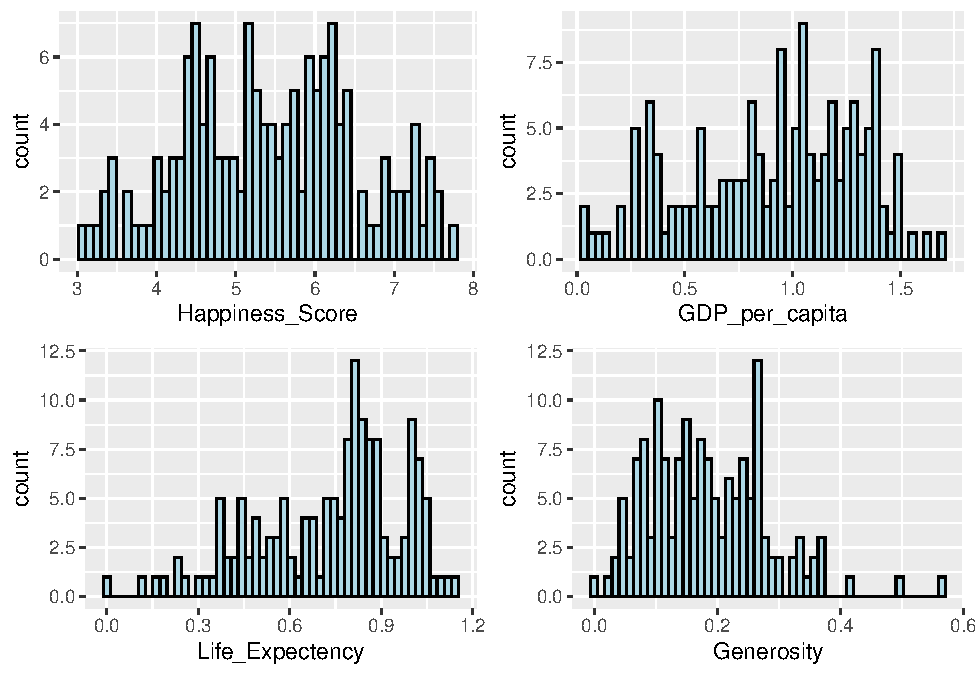
\includegraphics{World-Happiness_files/figure-latex/unnamed-chunk-2-1.pdf}

A slightly different look at the table grouped by regions.

\begin{verbatim}
## # A tibble: 10 x 5
##    Region                          mean_Score mean_GDP mean_LE mean_Generosity
##    <chr>                                <dbl>    <dbl>   <dbl>           <dbl>
##  1 Australia and New Zealand             7.27    1.34    1.03            0.331
##  2 Central and Eastern Europe            5.57    1.02    0.808           0.141
##  3 Eastern Asia                          5.69    1.24    0.953           0.173
##  4 Latin America and Caribbean           5.94    0.909   0.817           0.143
##  5 Middle East and Northern Africa       5.24    1.06    0.751           0.153
##  6 North America                         7.08    1.40    0.956           0.282
##  7 Southeastern Asia                     5.27    0.93    0.745           0.302
##  8 Southern Asia                         4.53    0.650   0.617           0.235
##  9 Sub-Saharan Africa                    4.31    0.452   0.412           0.187
## 10 Western Europe                        6.90    1.36    1.01            0.221
\end{verbatim}

\begin{verbatim}
## # A tibble: 10 x 5
##    Region                          mean_Score mean_GDP mean_LE mean_Generosity
##    <chr>                                <dbl>    <dbl>   <dbl>           <dbl>
##  1 Australia and New Zealand             7.28    1.29    0.920           0.455
##  2 Central and Eastern Europe            5.34    0.943   0.718           0.150
##  3 Eastern Asia                          5.63    1.15    0.877           0.226
##  4 Latin America and Caribbean           6.14    0.854   0.713           0.215
##  5 Middle East and Northern Africa       5.33    1.05    0.703           0.189
##  6 North America                         7.27    1.36    0.884           0.430
##  7 Southeastern Asia                     5.32    0.789   0.677           0.419
##  8 Southern Asia                         4.58    0.560   0.541           0.341
##  9 Sub-Saharan Africa                    4.17    0.370   0.277           0.218
## 10 Western Europe                        6.74    1.30    0.908           0.304
\end{verbatim}

\begin{center}\includegraphics[angle=90]{World-Happiness_files/figure-latex/unnamed-chunk-3-1} \end{center}

\hfill\break

\hypertarget{density-of-the-different-variables}{%
\paragraph{Density of the different
variables:}\label{density-of-the-different-variables}}

In order to be more confident about our distribution of the data, we
will use geom\_density function to visualize the bell shaped graph.

\begin{Shaded}
\begin{Highlighting}[]
\NormalTok{data\_density }\OtherTok{\textless{}{-}} \FunctionTok{ggplot}\NormalTok{(whr2019) }\SpecialCharTok{+}
  \FunctionTok{geom\_density}\NormalTok{(}\FunctionTok{aes}\NormalTok{(Happiness\_Score, }\AttributeTok{fill=}\StringTok{"Happiness score"}\NormalTok{, }\AttributeTok{alpha=}\FloatTok{0.1}\NormalTok{)) }\SpecialCharTok{+} 
  \FunctionTok{geom\_density}\NormalTok{(}\FunctionTok{aes}\NormalTok{(GDP\_per\_capita, }\AttributeTok{fill=}\StringTok{"GDP per capita"}\NormalTok{, }\AttributeTok{alpha=}\FloatTok{0.1}\NormalTok{)) }\SpecialCharTok{+} 
  \FunctionTok{geom\_density}\NormalTok{(}\FunctionTok{aes}\NormalTok{(Life\_Expectency, }\AttributeTok{fill=}\StringTok{"Life expectency"}\NormalTok{, }\AttributeTok{alpha=}\FloatTok{0.1}\NormalTok{)) }\SpecialCharTok{+} 
  \FunctionTok{geom\_density}\NormalTok{(}\FunctionTok{aes}\NormalTok{(Generosity, }\AttributeTok{fill=}\StringTok{"Generosity"}\NormalTok{, }\AttributeTok{alpha=}\FloatTok{0.1}\NormalTok{)) }\SpecialCharTok{+} 
    \FunctionTok{scale\_x\_continuous}\NormalTok{(}\AttributeTok{name =} \StringTok{"Variables"}\NormalTok{) }\SpecialCharTok{+}
  \FunctionTok{ggtitle}\NormalTok{(}\StringTok{"Distribution of the data"}\NormalTok{)}
  
\FunctionTok{plot}\NormalTok{(data\_density)}
\end{Highlighting}
\end{Shaded}

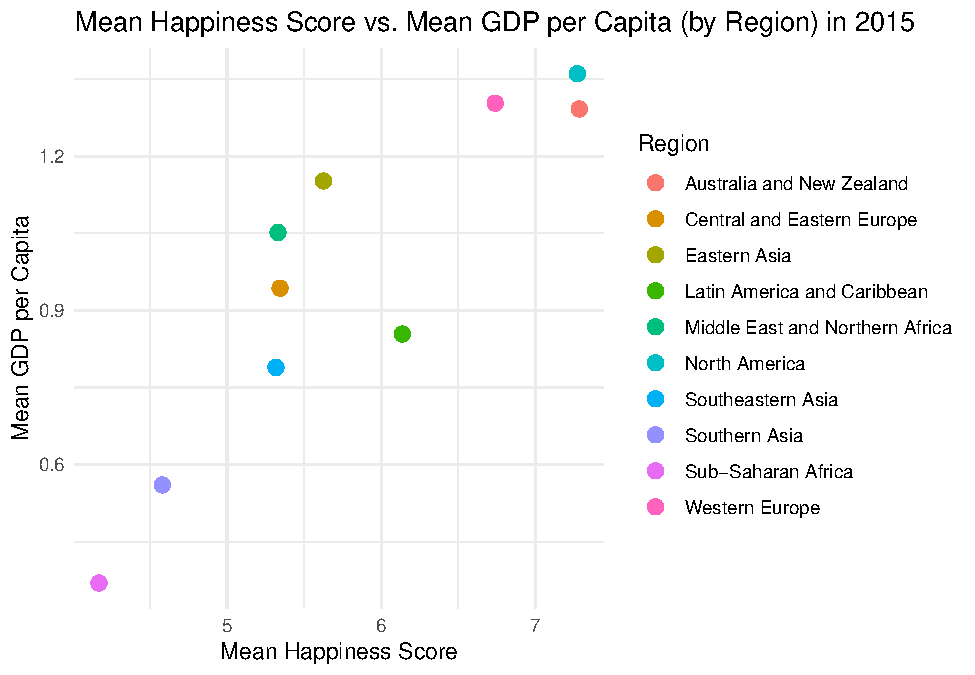
\includegraphics{World-Happiness_files/figure-latex/unnamed-chunk-4-1.pdf}

As we can see the different variables do have a bell shaped
distribution.

But to be even more confident we will now use QQPlot Graph.

\begin{Shaded}
\begin{Highlighting}[]
\NormalTok{happy\_qq }\OtherTok{\textless{}{-}} \FunctionTok{ggplot}\NormalTok{(whr2019, }\FunctionTok{aes}\NormalTok{(}\AttributeTok{sample=}\NormalTok{Happiness\_Score)) }\SpecialCharTok{+}
  \FunctionTok{geom\_qq}\NormalTok{(}\AttributeTok{color =} \StringTok{"honeydew3"}\NormalTok{) }\SpecialCharTok{+} \FunctionTok{geom\_qq\_line}\NormalTok{(}\AttributeTok{col=}\StringTok{"red"}\NormalTok{) }\SpecialCharTok{+} \FunctionTok{theme\_bw}\NormalTok{() }\SpecialCharTok{+}
    \FunctionTok{labs}\NormalTok{(}\AttributeTok{x=} \StringTok{"Happiness Score"}\NormalTok{) }

\NormalTok{gdp\_qq }\OtherTok{\textless{}{-}} \FunctionTok{ggplot}\NormalTok{(whr2019, }\FunctionTok{aes}\NormalTok{(}\AttributeTok{sample=}\NormalTok{GDP\_per\_capita)) }\SpecialCharTok{+}
  \FunctionTok{geom\_qq}\NormalTok{(}\AttributeTok{color =} \StringTok{"honeydew3"}\NormalTok{) }\SpecialCharTok{+} \FunctionTok{geom\_qq\_line}\NormalTok{(}\AttributeTok{col=}\StringTok{"red"}\NormalTok{) }\SpecialCharTok{+}\FunctionTok{theme\_bw}\NormalTok{() }\SpecialCharTok{+}
    \FunctionTok{labs}\NormalTok{(}\AttributeTok{x=} \StringTok{"GDP per capita"}\NormalTok{)}

\NormalTok{life\_expectency\_qq }\OtherTok{\textless{}{-}} \FunctionTok{ggplot}\NormalTok{(whr2019, }\FunctionTok{aes}\NormalTok{(}\AttributeTok{sample=}\NormalTok{Life\_Expectency)) }\SpecialCharTok{+}
  \FunctionTok{geom\_qq}\NormalTok{(}\AttributeTok{color =} \StringTok{"honeydew3"}\NormalTok{) }\SpecialCharTok{+} \FunctionTok{geom\_qq\_line}\NormalTok{(}\AttributeTok{col=}\StringTok{"red"}\NormalTok{) }\SpecialCharTok{+} \FunctionTok{theme\_bw}\NormalTok{() }\SpecialCharTok{+}
    \FunctionTok{labs}\NormalTok{(}\AttributeTok{x=} \StringTok{"Life Expectency"}\NormalTok{)}

\NormalTok{generosity\_qq }\OtherTok{\textless{}{-}} \FunctionTok{ggplot}\NormalTok{(whr2019, }\FunctionTok{aes}\NormalTok{(}\AttributeTok{sample=}\NormalTok{Generosity)) }\SpecialCharTok{+}
  \FunctionTok{geom\_qq}\NormalTok{(}\AttributeTok{color =} \StringTok{"honeydew3"}\NormalTok{) }\SpecialCharTok{+} \FunctionTok{geom\_qq\_line}\NormalTok{(}\AttributeTok{col=}\StringTok{"red"}\NormalTok{) }\SpecialCharTok{+} \FunctionTok{theme\_bw}\NormalTok{() }\SpecialCharTok{+}
    \FunctionTok{labs}\NormalTok{(}\AttributeTok{x=} \StringTok{"Generosity"}\NormalTok{)}

\FunctionTok{grid.arrange}\NormalTok{(happy\_qq, gdp\_qq,life\_expectency\_qq,generosity\_qq)}
\end{Highlighting}
\end{Shaded}

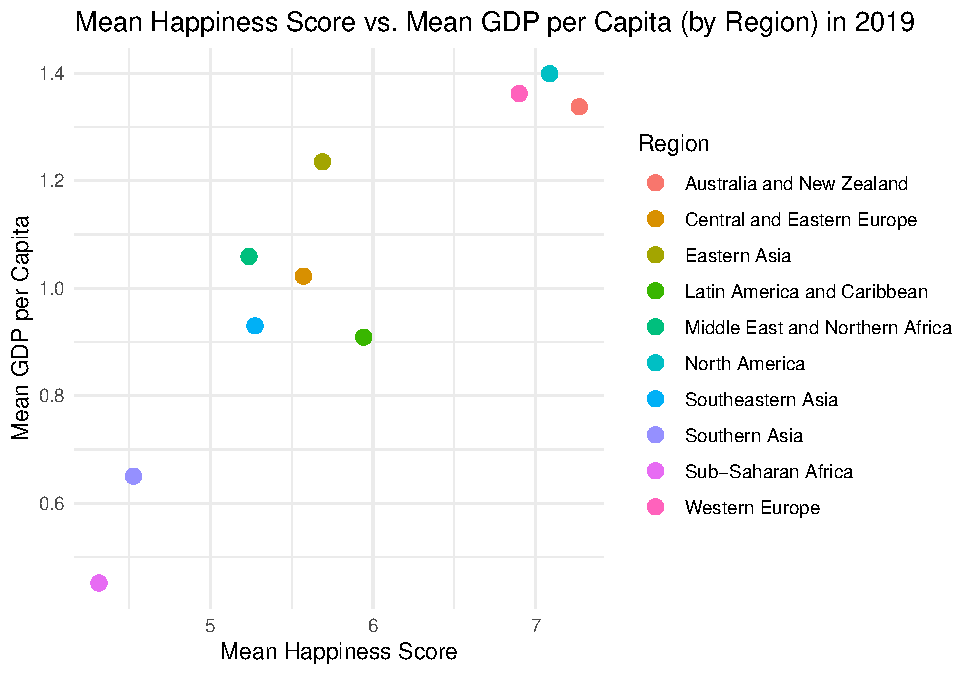
\includegraphics{World-Happiness_files/figure-latex/unnamed-chunk-5-1.pdf}

From these graphs we could be pretty sure that our data is indeed
normally distributed.

Lets take a look on the happiness score with boxplot.

\begin{Shaded}
\begin{Highlighting}[]
\FunctionTok{boxplot}\NormalTok{(whr2015}\SpecialCharTok{$}\NormalTok{Happiness\_Score, whr2019}\SpecialCharTok{$}\NormalTok{Happiness\_Score,}
        \AttributeTok{names =} \FunctionTok{c}\NormalTok{(}\StringTok{"2015"}\NormalTok{, }\StringTok{"2019"}\NormalTok{))}
\end{Highlighting}
\end{Shaded}

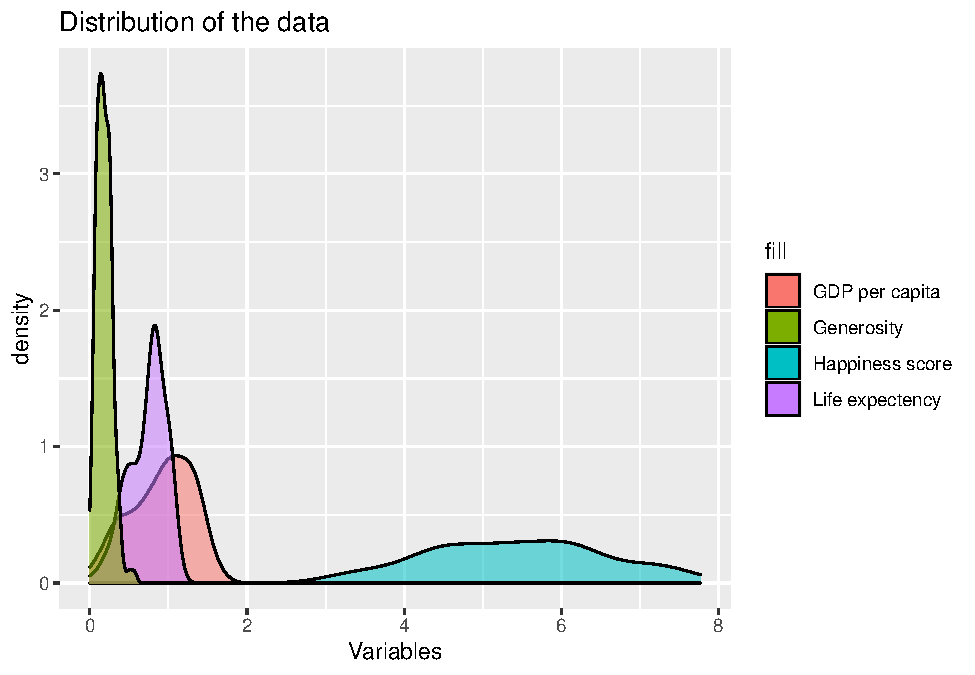
\includegraphics{World-Happiness_files/figure-latex/unnamed-chunk-6-1.pdf}\\

Using geometric points to draw a conclusion about the level of happiness
and GDP product by regions.

We can understand which areas have a higher level of happiness and
product.

\begin{Shaded}
\begin{Highlighting}[]
\FunctionTok{ggplot}\NormalTok{(whr2015) }\SpecialCharTok{+} \FunctionTok{geom\_point}\NormalTok{(}\FunctionTok{aes}\NormalTok{(}\AttributeTok{x =}\NormalTok{ Happiness\_Score, }\AttributeTok{y =}\NormalTok{ GDP\_per\_capita, }\AttributeTok{color =}\NormalTok{ Region))}
\end{Highlighting}
\end{Shaded}

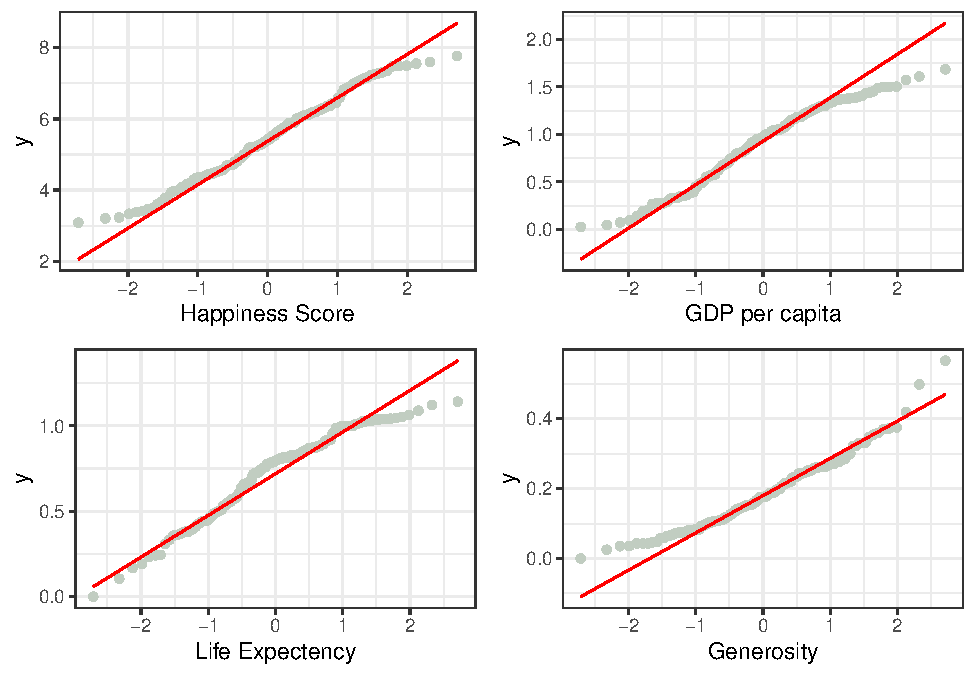
\includegraphics{World-Happiness_files/figure-latex/unnamed-chunk-7-1.pdf}

Western Europe as a group has the higher level of Happiness score and
GDP.

On the other hand Sub-Saharan Africa has the lower level of Happiness
and GDP.

\hfill\break

\hypertarget{modeling}{%
\subsubsection{Modeling}\label{modeling}}

After we got to know our data better we can now move on to carry out our
research.

\hypertarget{hypothesis-test---difference-in-means.}{%
\paragraph{1. Hypothesis test - difference in
means.}\label{hypothesis-test---difference-in-means.}}

The happiness index in the world is expected to be the same. We will
perform a system of hypotheses to test whether the happiness score has
increased over the years and the world is moving towards a better
future.

Since we compare two samples with the same parameters we will conduct a
paired t-test. Therefore our samples are paired samples.

\(\mu_{1}\): The average score of 2019 report\\
\(\mu_{2}\): The average score of 2015 report\\
\strut \\

Hypothesis test:

\(H_{0}: \mu_{1}-\mu_{2} = 0\)\\
\(H_{1}: \mu_{1}-\mu_{2} > 0\)\\

\begin{Shaded}
\begin{Highlighting}[]
\FunctionTok{t.test}\NormalTok{(whr2019}\SpecialCharTok{$}\NormalTok{Happiness\_Score, whr2015}\SpecialCharTok{$}\NormalTok{Happiness\_Score, }\AttributeTok{paired =} \ConstantTok{TRUE}\NormalTok{, }
       \AttributeTok{alternative =} \StringTok{"greater"}\NormalTok{)}
\end{Highlighting}
\end{Shaded}

\begin{verbatim}
## 
##  Paired t-test
## 
## data:  whr2019$Happiness_Score and whr2015$Happiness_Score
## t = 0.96123, df = 148, p-value = 0.169
## alternative hypothesis: true difference in means is greater than 0
## 95 percent confidence interval:
##  -0.04013068         Inf
## sample estimates:
## mean of the differences 
##              0.05558389
\end{verbatim}

\hypertarget{conclusion}{%
\paragraph{Conclusion:}\label{conclusion}}

We thought that the overall happiness will increase over the years. We
compared P.value to the alpha value and saw that Alpha \textless{}
P.Value therefore we will not reject the null hypothesis. Therefore, the
differences between the two years are insignificant. We will conclude
that there has been no significant change in the level of happiness in
the world.

\hfill\break

\hypertarget{multiple-regression}{%
\paragraph{2. Multiple Regression}\label{multiple-regression}}

First, we want to see the correlation between the different variables
and find simple association rules.

\begin{Shaded}
\begin{Highlighting}[]
\NormalTok{numberic\_whr }\OtherTok{\textless{}{-}}\NormalTok{ whr2019 }\SpecialCharTok{\%\textgreater{}\%}
  \FunctionTok{select}\NormalTok{(Happiness\_Score, GDP\_per\_capita, Life\_Expectency, Freedom, Generosity, Corruption)}

\NormalTok{whr\_corr }\OtherTok{\textless{}{-}} \FunctionTok{cor}\NormalTok{(numberic\_whr)}

\FunctionTok{ggcorrplot}\NormalTok{(whr\_corr, }\AttributeTok{hc.order =} \ConstantTok{TRUE}\NormalTok{, }\AttributeTok{type =} \StringTok{"upper"}\NormalTok{, }\AttributeTok{lab =}\NormalTok{ T,}
           \AttributeTok{ggtheme =}\NormalTok{ ggplot2}\SpecialCharTok{::}\NormalTok{theme\_gray)}
\end{Highlighting}
\end{Shaded}

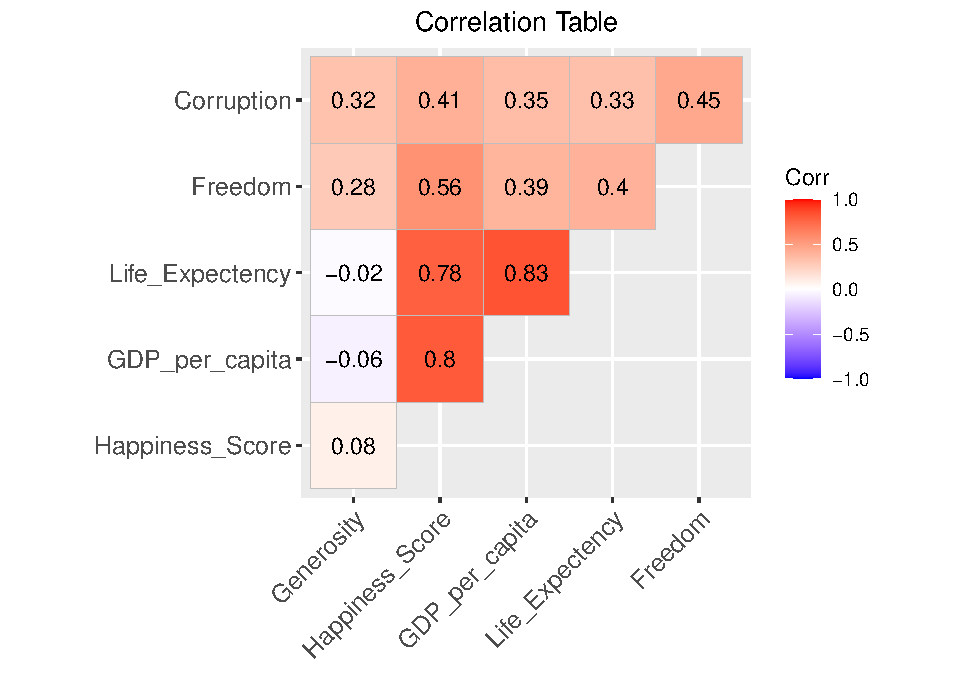
\includegraphics{World-Happiness_files/figure-latex/unnamed-chunk-9-1.pdf}\\

We can conclude from the chart that there is a high correlation between
Happiness score, life expectancy and the GDP index. That is, there is an
almost perfect match between these three variables.

Moreover, we can infer that the level of generosity in countries has
almost no effect on the life expectancy and the GDP per capita.\\
\strut \\

Now we can create the linear model using Summary Statistics Table:

\begin{Shaded}
\begin{Highlighting}[]
\NormalTok{model }\OtherTok{\textless{}{-}} \FunctionTok{lm}\NormalTok{(Happiness\_Score }\SpecialCharTok{\textasciitilde{}}\NormalTok{ GDP\_per\_capita }\SpecialCharTok{+}\NormalTok{ Life\_Expectency }\SpecialCharTok{+}\NormalTok{ Freedom }\SpecialCharTok{+} 
\NormalTok{              Generosity }\SpecialCharTok{+}\NormalTok{ Corruption, }\AttributeTok{data =}\NormalTok{ whr2019)}
\FunctionTok{summary}\NormalTok{(model)}
\end{Highlighting}
\end{Shaded}

\begin{verbatim}
## 
## Call:
## lm(formula = Happiness_Score ~ GDP_per_capita + Life_Expectency + 
##     Freedom + Generosity + Corruption, data = whr2019)
## 
## Residuals:
##      Min       1Q   Median       3Q      Max 
## -1.85095 -0.33158  0.08602  0.39151  0.97172 
## 
## Coefficients:
##                 Estimate Std. Error t value Pr(>|t|)    
## (Intercept)       2.3842     0.1924  12.394  < 2e-16 ***
## GDP_per_capita    1.2228     0.2222   5.503 1.67e-07 ***
## Life_Expectency   1.4688     0.3603   4.076 7.57e-05 ***
## Freedom           1.8372     0.4015   4.575 1.02e-05 ***
## Generosity        0.4582     0.5427   0.844    0.400    
## Corruption        0.4427     0.5945   0.745    0.458    
## ---
## Signif. codes:  0 '***' 0.001 '**' 0.01 '*' 0.05 '.' 0.1 ' ' 1
## 
## Residual standard error: 0.5764 on 143 degrees of freedom
## Multiple R-squared:   0.74,  Adjusted R-squared:  0.7309 
## F-statistic:  81.4 on 5 and 143 DF,  p-value: < 2.2e-16
\end{verbatim}

The first step in interpreting the multiple regression analysis is to
examine the F-statistic and the associated p-value, at the bottom of
model summary.

In this model, it can be seen that p-value of the F-statistic is
\textless{} 2.2e-16, which is highly significant. This means that, at
least, one of the predictor variables is significantly related to the
outcome variable.

By looking at the coefficients table of the variables we can see that
there is significant association between GDP per capita, life expectancy
and freedom with the outcome variable - the happiness score.

But, generosity and corruption variables are not significant in the
model.

Which means that the 74\% of the score of happiness can explained by
these variables.\\

Because generosity and corruption are not significant we can remove them
from the model and get even more accurate model:

\begin{Shaded}
\begin{Highlighting}[]
\NormalTok{model2 }\OtherTok{\textless{}{-}} \FunctionTok{lm}\NormalTok{(Happiness\_Score }\SpecialCharTok{\textasciitilde{}}\NormalTok{ GDP\_per\_capita }\SpecialCharTok{+}\NormalTok{ Life\_Expectency }\SpecialCharTok{+}\NormalTok{ Freedom, }\AttributeTok{data =}\NormalTok{ whr2019)}
\FunctionTok{summary}\NormalTok{(model2)}
\end{Highlighting}
\end{Shaded}

\begin{verbatim}
## 
## Call:
## lm(formula = Happiness_Score ~ GDP_per_capita + Life_Expectency + 
##     Freedom, data = whr2019)
## 
## Residuals:
##      Min       1Q   Median       3Q      Max 
## -1.93954 -0.36786  0.05693  0.41276  1.02537 
## 
## Coefficients:
##                 Estimate Std. Error t value Pr(>|t|)    
## (Intercept)       2.4297     0.1745  13.926  < 2e-16 ***
## GDP_per_capita    1.2172     0.2178   5.589 1.10e-07 ***
## Life_Expectency   1.4783     0.3599   4.107 6.66e-05 ***
## Freedom           2.0558     0.3655   5.625 9.25e-08 ***
## ---
## Signif. codes:  0 '***' 0.001 '**' 0.01 '*' 0.05 '.' 0.1 ' ' 1
## 
## Residual standard error: 0.576 on 145 degrees of freedom
## Multiple R-squared:  0.7368, Adjusted R-squared:  0.7314 
## F-statistic: 135.3 on 3 and 145 DF,  p-value: < 2.2e-16
\end{verbatim}

As expected the R-Squared went down by a small amount since we dropped
two variables from the model. Also, the Adjusted R-Squared indeed went
up (the closer to 1 the better).\\

Let's take a look on the linear regression of each variable with the
happiness score:

\begin{Shaded}
\begin{Highlighting}[]
\NormalTok{gg\_hs\_gdp }\OtherTok{\textless{}{-}} \FunctionTok{ggplot}\NormalTok{(whr2019, }\FunctionTok{aes}\NormalTok{(}\AttributeTok{x=}\NormalTok{GDP\_per\_capita, }\AttributeTok{y=}\NormalTok{Happiness\_Score)) }\SpecialCharTok{+}
  \FunctionTok{geom\_point}\NormalTok{() }\SpecialCharTok{+}
  \FunctionTok{stat\_smooth}\NormalTok{(}\AttributeTok{method =} \StringTok{"lm"}\NormalTok{)}

\NormalTok{gg\_hs\_le }\OtherTok{\textless{}{-}} \FunctionTok{ggplot}\NormalTok{(whr2019, }\FunctionTok{aes}\NormalTok{(}\AttributeTok{x=}\NormalTok{Life\_Expectency, }\AttributeTok{y=}\NormalTok{Happiness\_Score)) }\SpecialCharTok{+}
  \FunctionTok{geom\_point}\NormalTok{() }\SpecialCharTok{+}
  \FunctionTok{stat\_smooth}\NormalTok{(}\AttributeTok{method =} \StringTok{"lm"}\NormalTok{)}

\NormalTok{gg\_hs\_free }\OtherTok{\textless{}{-}} \FunctionTok{ggplot}\NormalTok{(whr2019, }\FunctionTok{aes}\NormalTok{(}\AttributeTok{x=}\NormalTok{Freedom, }\AttributeTok{y=}\NormalTok{Happiness\_Score)) }\SpecialCharTok{+}
  \FunctionTok{geom\_point}\NormalTok{() }\SpecialCharTok{+}
  \FunctionTok{stat\_smooth}\NormalTok{(}\AttributeTok{method =} \StringTok{"lm"}\NormalTok{)}

\NormalTok{gg\_hs\_genr }\OtherTok{\textless{}{-}} \FunctionTok{ggplot}\NormalTok{(whr2019, }\FunctionTok{aes}\NormalTok{(}\AttributeTok{x=}\NormalTok{Generosity, }\AttributeTok{y=}\NormalTok{Happiness\_Score)) }\SpecialCharTok{+}
  \FunctionTok{geom\_point}\NormalTok{() }\SpecialCharTok{+}
  \FunctionTok{stat\_smooth}\NormalTok{(}\AttributeTok{method =} \StringTok{"lm"}\NormalTok{)}

\NormalTok{gg\_hs\_corr }\OtherTok{\textless{}{-}} \FunctionTok{ggplot}\NormalTok{(whr2019, }\FunctionTok{aes}\NormalTok{(}\AttributeTok{x=}\NormalTok{Corruption, }\AttributeTok{y=}\NormalTok{Happiness\_Score)) }\SpecialCharTok{+}
  \FunctionTok{geom\_point}\NormalTok{() }\SpecialCharTok{+}
  \FunctionTok{stat\_smooth}\NormalTok{(}\AttributeTok{method =} \StringTok{"lm"}\NormalTok{)}

\FunctionTok{grid.arrange}\NormalTok{(gg\_hs\_gdp, gg\_hs\_le, gg\_hs\_free, gg\_hs\_genr, gg\_hs\_corr)}
\end{Highlighting}
\end{Shaded}

\includegraphics{World-Happiness_files/figure-latex/unnamed-chunk-12-1.pdf}\\

As observed and stated before GDP per capita, life expectancy and
freedom are indeed correlated to the happiness score, whereas generosity
and corruption are not that correlated\ldots{}

But before even making final conclusions we must first check whether our
model does meet the assumptions:\\
- The residuals are homoscedastic.\\
- The residuals are distributed normally.\\
- No multicollinearity between the explanatory variables.\\
\strut \\

\hypertarget{residual-plot}{%
\paragraph{Residual Plot}\label{residual-plot}}

\begin{Shaded}
\begin{Highlighting}[]
\NormalTok{residual\_upd\_model }\OtherTok{\textless{}{-}}\NormalTok{ model2}\SpecialCharTok{$}\NormalTok{residuals}

\NormalTok{model2 }\SpecialCharTok{\%\textgreater{}\%} \FunctionTok{ggplot}\NormalTok{(}\FunctionTok{aes}\NormalTok{(}\AttributeTok{x=}\NormalTok{.fitted,}\AttributeTok{y=}\NormalTok{.resid)) }\SpecialCharTok{+}
  \FunctionTok{geom\_point}\NormalTok{() }\SpecialCharTok{+} \FunctionTok{geom\_hline}\NormalTok{(}\AttributeTok{yintercept=}\DecValTok{0}\NormalTok{) }\SpecialCharTok{+}
  \FunctionTok{labs}\NormalTok{(}\AttributeTok{title=}\StringTok{"Residual Plot"}\NormalTok{)}
\end{Highlighting}
\end{Shaded}

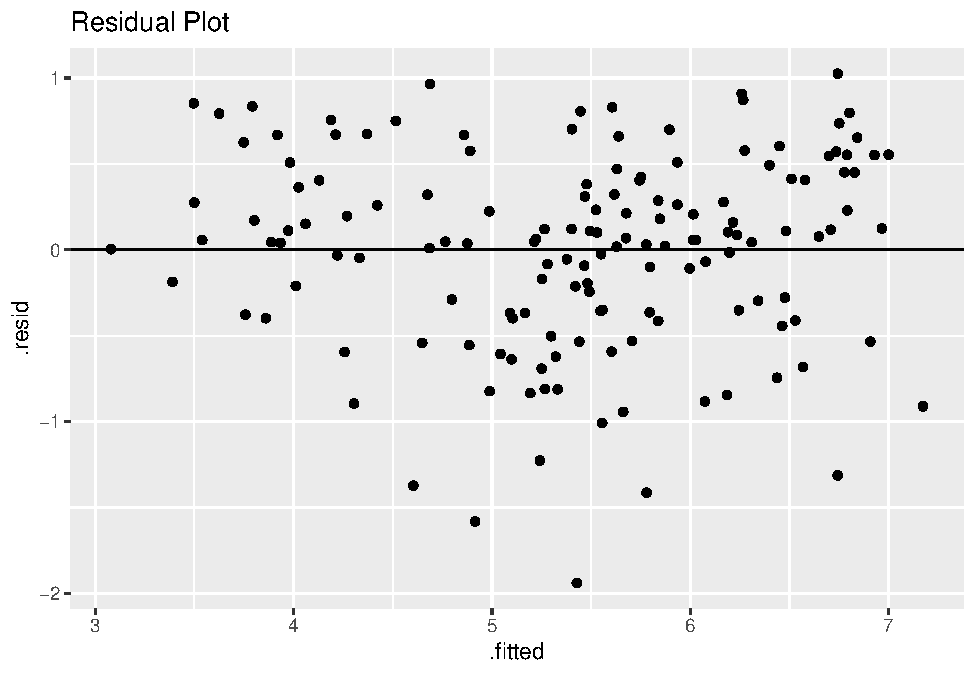
\includegraphics{World-Happiness_files/figure-latex/unnamed-chunk-13-1.pdf}\\
\strut \\

\hypertarget{distribution-of-the-residuals-using-qq-plot}{%
\paragraph{Distribution of the residuals using QQ
Plot}\label{distribution-of-the-residuals-using-qq-plot}}

\begin{Shaded}
\begin{Highlighting}[]
\NormalTok{model2 }\SpecialCharTok{\%\textgreater{}\%} \FunctionTok{ggplot}\NormalTok{(}\FunctionTok{aes}\NormalTok{(}\AttributeTok{sample=}\NormalTok{.resid)) }\SpecialCharTok{+}
  \FunctionTok{geom\_qq}\NormalTok{() }\SpecialCharTok{+} \FunctionTok{geom\_qq\_line}\NormalTok{(}\AttributeTok{col=}\StringTok{"red"}\NormalTok{) }\SpecialCharTok{+}
  \FunctionTok{labs}\NormalTok{(}\AttributeTok{title=}\StringTok{"QQ Plot"}\NormalTok{)}
\end{Highlighting}
\end{Shaded}

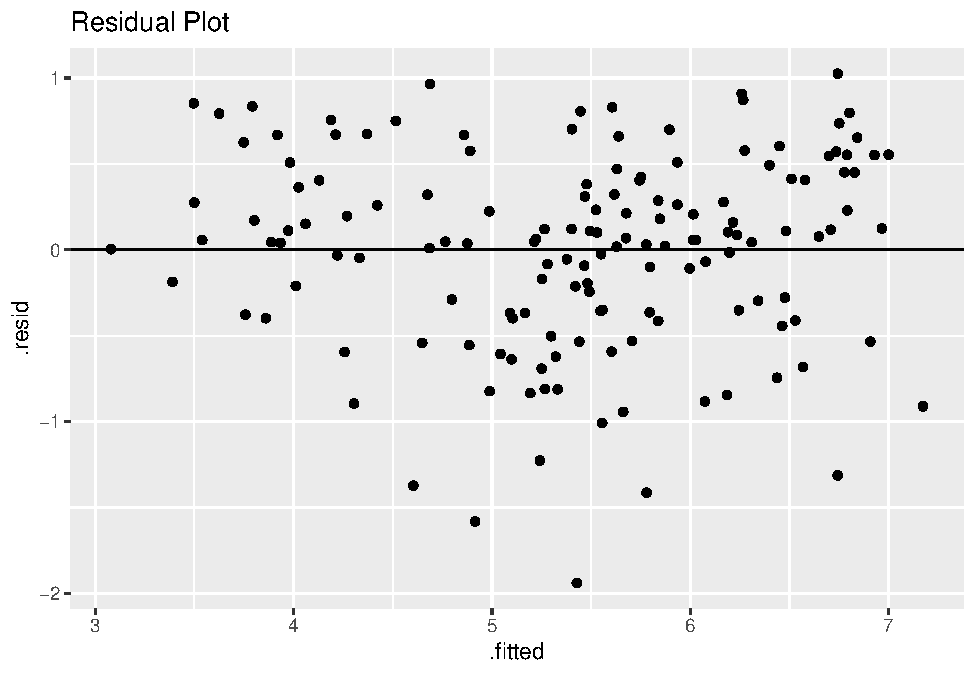
\includegraphics{World-Happiness_files/figure-latex/unnamed-chunk-14-1.pdf}\\
\strut \\

\hypertarget{vif-between-the-explanatory-variables}{%
\paragraph{VIF between the explanatory
variables}\label{vif-between-the-explanatory-variables}}

\begin{Shaded}
\begin{Highlighting}[]
\NormalTok{car}\SpecialCharTok{::}\FunctionTok{vif}\NormalTok{(model2)}
\end{Highlighting}
\end{Shaded}

\begin{verbatim}
##  GDP_per_capita Life_Expectency         Freedom 
##        3.262036        3.288904        1.206238
\end{verbatim}

\hfill\break

As we can see:

\begin{itemize}
\tightlist
\item
  the residuals are hetroscedastic\\
\item
  the residuals are not distributed normally\\
\item
  the VIF between the independent variables is lower than 5 which means
  they are not correlated.\\
\end{itemize}

It can be seen that assumptions 1 and 2 do not hold, therefore, the
model we have created seems to be unsuitable for predicting models.\\

\hypertarget{conclusion-1}{%
\subsubsection{Conclusion:}\label{conclusion-1}}

In the project we wanted to study the happiness index in the countries
of the world. We selected a database, presented the results and
researched them. We studied the variables in each country and their
effects on the happiness index. We used a number of models, among them -
Examining hypotheses for the level of happiness between different
countries over the years. A linear and multiple regression model on the
dependence of the happiness index on the explanatory variables, and on
the effect of different variables on the other data.

We have come to interesting conclusions about the different countries of
the world, the index of happiness in them and the variables that affect
and are affected by happiness.

The project helped us to understand in depth the different tests we
learned during the course, how to build them, how to work with them and
most importantly how to draw interesting conclusions from them.

\hfill\break
\hfill\break


\includegraphics{C:/Users/eitan/OneDrive/Desktop/TAU/Semester B/Statistics and Data Analysis/Happiness/Finding-Happiness.jpg}

\end{document}
